\chapter{Applications}
A lot of physics problems or application can be uniformly studied under the framework introduced in the previous chapters. However, for a specific problem, there are still many factors need to be considered. In this chapter, we will introduce the background of each specific problem, its special treatments as well as the implementations.
\section{Parachute Simulation}
Parachute simulation is a complex system coupling many aspects such as 
elastic mechanics and fluid dynamics. Therefore, a desirable implementation should include decoupled modules handling fluid dynamics, elastic mechanics as well as their interactions. We have developed a novel particle-based cloth model to mimic the in-plane energy by introducing the concept of angular stiffness. This model is then coupled with fluid dynamics through impulse method. In order to better simulate the turbulence effects, a zero-equation turbulence model is replaced with a two-equation model. We also proposed a new 
porosity model for the fabric surface to consider the porosity effects. 
In addition, a new collision handling function is developed to efficiently and 
robustly treat the collision among fabric surface, rigid body and suspension lines.

\subsection{Model Description}
The mathematics model of the parachute simulation follows the framework in Chapter \ref{background}. The hydrodynamic behavior of a turbulent incompressible fluid is governed by the RANS equations for the mean velocity and pressure. We still consider the $k-\varepsilon$ family as the turbulence model, which automatically
calculate the turbulence length scale \cite{wilcox1998turbulence}.  In standard
$k-\varepsilon$ model, the eddy viscosity is defined as 
\begin{equation} \nu_T =
C_{\mu}\frac{k^2}{\varepsilon}, \label{eq:nuT} 
\end{equation} 
where $k$ is the turbulence kinetic energy and $\varepsilon$ is the dissipation rate. To compute $k$ and $\varepsilon$, two additional convection-diffusion-reaction equations
are needed: 
\begin{equation} 
\frac{\partial k}{\partial
t}+\nabla\cdot(kU-(\nu+\frac{\nu_T}{\delta_k})\nabla k) =P_k - \varepsilon
\label{eq:k} 
\end{equation} 

\begin{equation} \frac{\partial
\varepsilon}{\partial t}+\nabla\cdot(\varepsilon U
-(\nu+\frac{\nu_T}{\delta_\varepsilon})\nabla \varepsilon)
=\frac{\varepsilon}{k}(C_1P_k-C_2\varepsilon) \label{eq:eps} 
\end{equation}
where $P_k = \frac{\nu_T}{2}|\nabla U + \nabla U^T|^2$ is the production of
turbulent kinetic energy. For the standard $k-\varepsilon$ model, the default
values of the involved empirical constants are: $C_\mu = 0.09$, $C_1 = 1.44$,
$C_2=1.92$, $\delta_k=1.0$, $\delta_{\varepsilon}=1.3$.  Although simple and
efficient, the standard model is unable to capture the effects of smaller scales
of motion due to its single turbulence length scale.  In order to account for
the different scales of motion, a mathematical technique called Re-Normalization
Group (RNG) method \cite{yakhot1992renormalization} is used to derive a
turbulence model similar to the standard one, resulting in a modified form of
the $\varepsilon$ equation: 
\begin{equation} 
\frac{\partial
\varepsilon}{\partial t}+\nabla\cdot(\varepsilon U
-(\nu+\frac{\nu_T}{\delta_\varepsilon})\nabla \varepsilon)
=\frac{\varepsilon}{k}(C_1P_k-C^*_2\varepsilon) \label{eq:RNG} 
\end{equation}

\begin{equation} 
C^*_2=C_2+\frac{C_{\mu}\eta^3(1-\eta/\eta_0)}{1+\beta\eta^3}
\end{equation} 
$\eta = kS/\varepsilon$, $S$ is the modulus of the mean rate of
strain tensor.  The coefficients are derived explicitly in the RNG procedure and
for completeness, we list here as: $C_\mu = 0.0845$, $C_1 = 1.42$, $C_2=1.68$,
$\delta_k=0.7194$, $\delta_{\varepsilon}=0.7194$. Figure \ref{fig:keps} displays the
viscosity and velocity streamline computed with RNG $k-\varepsilon$ model.

\begin{figure}[!ht] \centering \begin{tabular}{cc}
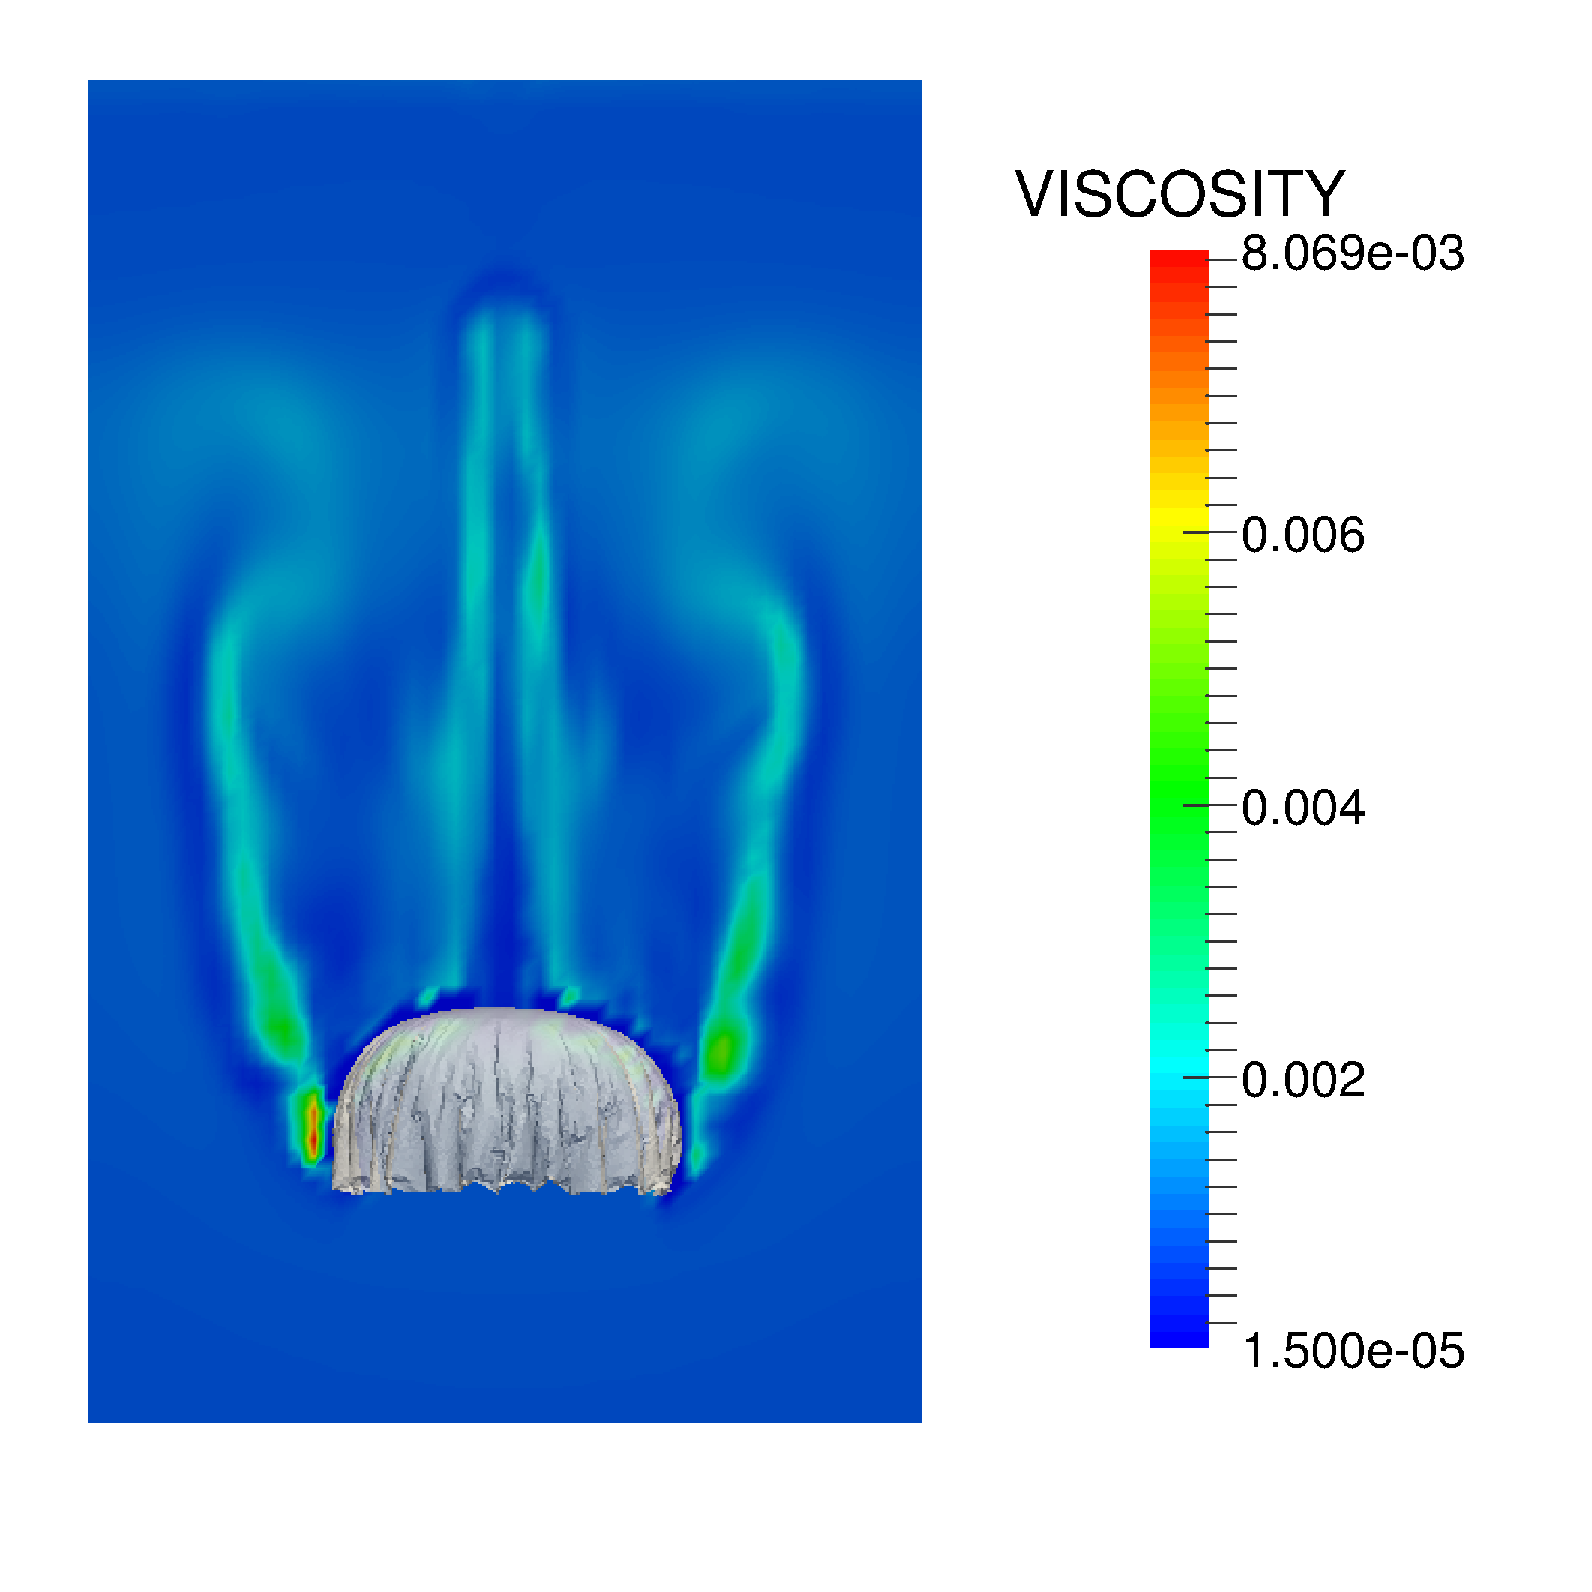
\epsfig{file=Figures/viscosity_rng,width=0.45\hsize} &
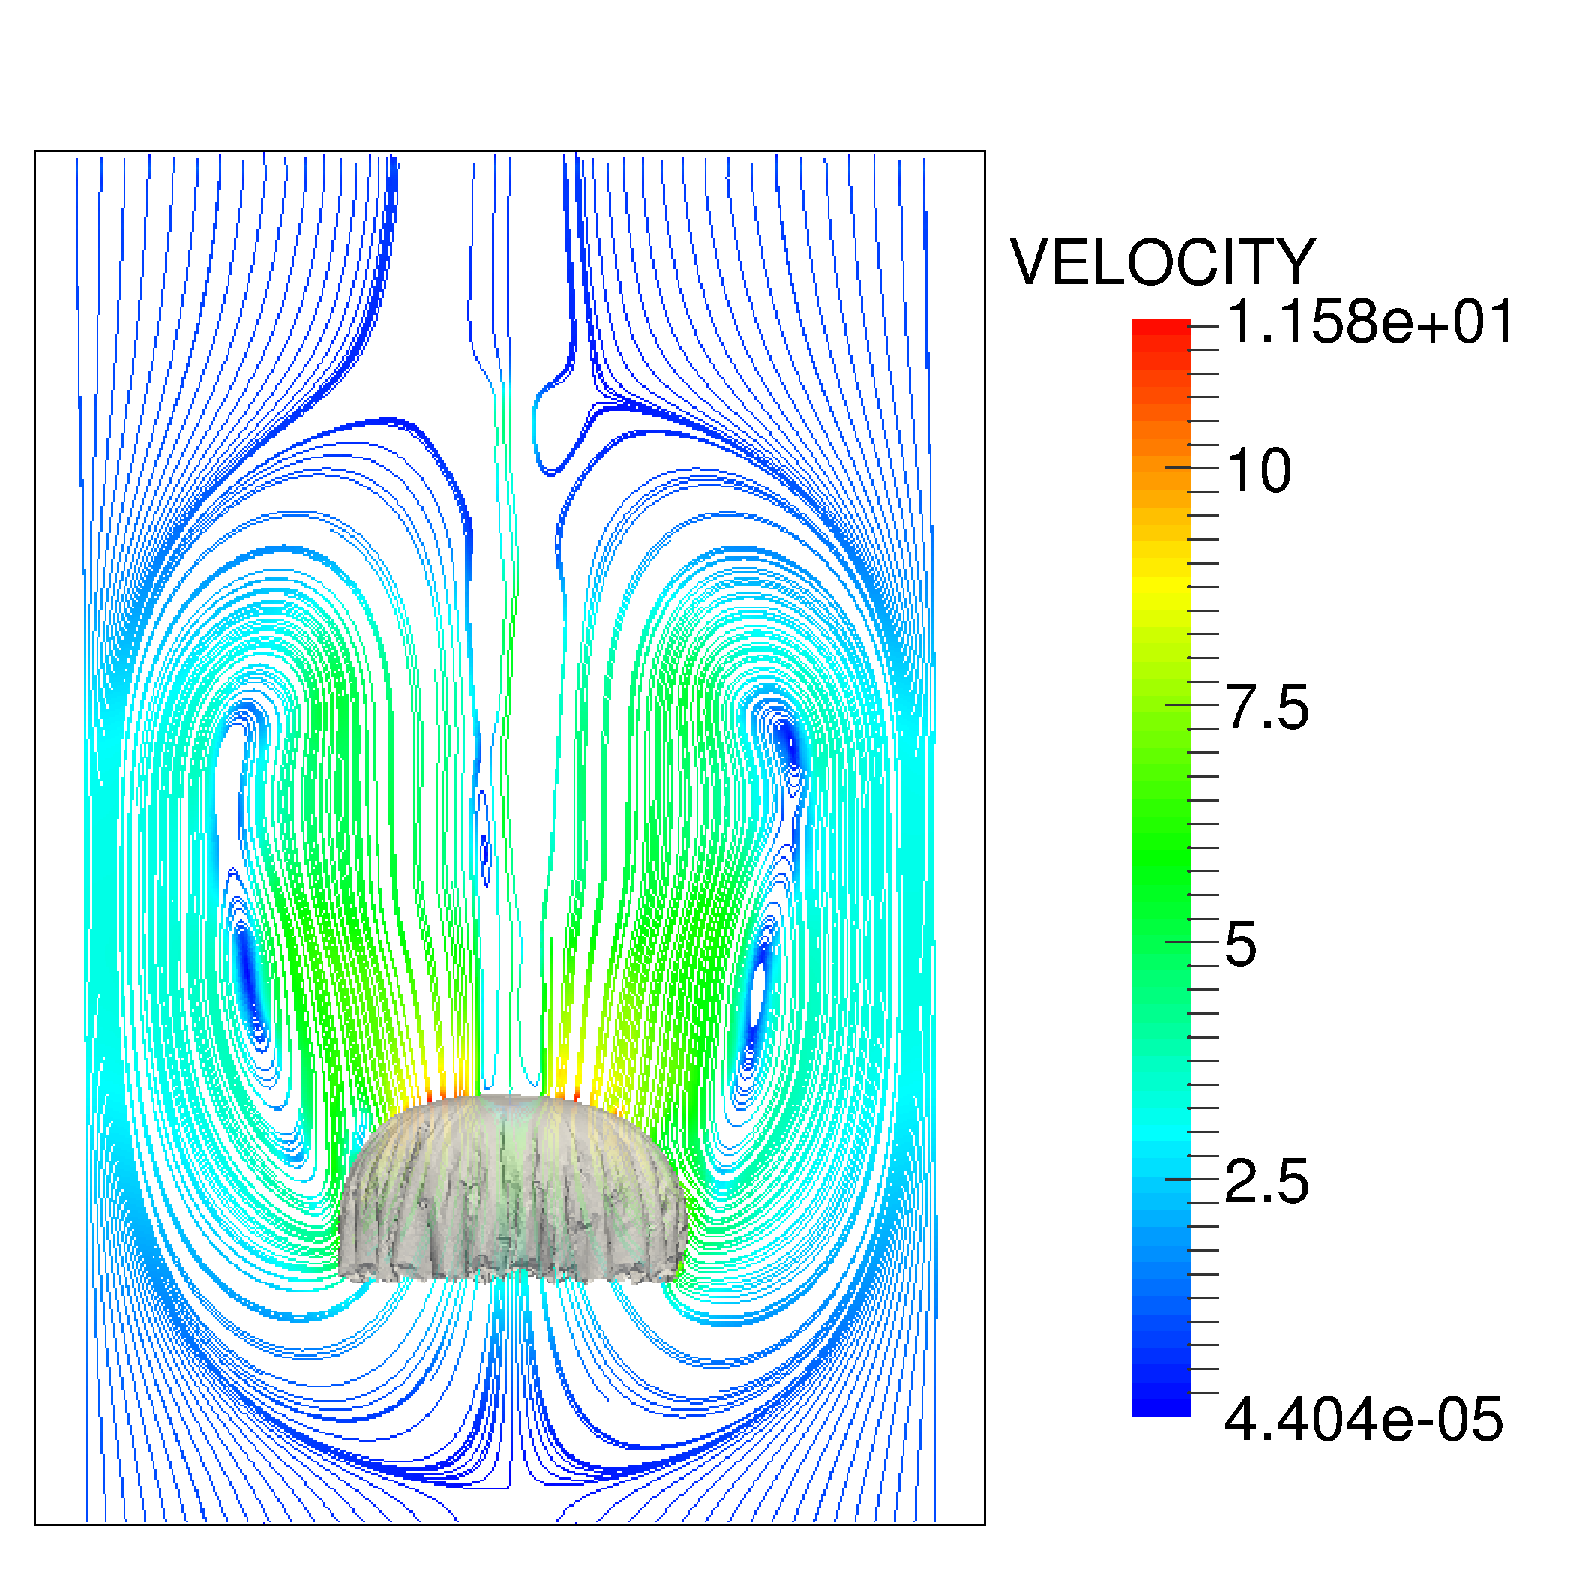
\epsfig{file=Figures/streamline_rng,width=0.45\hsize} \end{tabular}
\caption{Viscosity and streamline around parachute computed by RNG
$k-\varepsilon$ model \label{fig:keps}} \end{figure}

Modeling of fabric surface also poses many challenges. 
A fabric surface may fold and wrinkle, thus making it
difficult to model than an elastic plate. We proposed a mesoscale model using
the spring-mass system and strengthened it by the inclusion of both tensile and
angular stiffness, a model originally proposed by Delingette \cite{Delinget2008}.
The mathematics model for $n$ particles system is formulated as \ref{dv_eqn} and \ref{dx_eqn}. In our new spring mass model, the formula for computing the force is:
\begin{equation}
\vect{f} = -\frac{\partial W}{\partial \vect{x}} 
				+ \vect{f}_d + \vect{f}_e
\end{equation} 

This model is well defined except the energy function $W$ for each mass point. In fact, the elastic membrane can be discretized into triangles and then the potential energy in a deformed triangle consists of two parts: the energy of three tensile springs that prevent edges from stretching; the energy of three angular springs that prevent any change of vertex angles. 

In the following section, $W(T_p)$ is used to present the energy necessary to deform a triangle $T_{P_0}$ consisting of vertices $\{\vect{P}_{1,0}, \vect{P}_{2,0}, \vect{P}_{3,0}\}$ into  its deformed position $T_P$ with vertices $\{\vect{P}_{1}, \vect{P}_{2}, \vect{P}_{3}\}$; $l_{ij}$ and $l_{ij}^0$ denote the current and original length between vertex $\vect{P}_i$ and $\vect{P}_j$ respectively; $d_{ij}$ represents the edge elongation $dl_{ij} = l_{ij}-l_{ij}^0$. The potential energy for a single triangle is then given as \cite{Delinget2008} 

\[
W(T_{P})=\sum_{\substack{i=1, j \neq i}}^{3}\frac{1}{2}\kappa_{ij}^{T_{P_0}}
(dl_{ij})^{2}+\sum_{\substack{i=1, j \neq i \\ k \neq i, k \neq j}}^{3}\gamma_{i}^{T_{P_0}}dl_{ij}dl_{ik} 
\]

where \[
\kappa_{ij}^{T_{P_0}}=\frac{(l_{ij}^{0})^{2}(2\cot^{2}\alpha_{k}
(\lambda+\mu)+\mu)}{8A_{P_0}} \] 
is the tensile stiffness and
\begin{equation}
\gamma_{i}^{T_{P_0}}=\frac{l_{ik}^{0}l_{ij}^{0}(2\cot\alpha_{j}
\cot\alpha_{k}(\lambda+\mu)-\mu)}{8A_{P_0}} \label{eq:angular_stiff}
\end{equation} 
is the angular stiffness; $\alpha_j$ is the vertex angle in the undeformed triangle; $A_{P_0}$ is the area of triangle $T_{P_0}$. $\gamma$ and $\mu$ are the Lam\'{e}
coefficients of the material.  These coefficients are simply related to the
physically meaningful parameters for elastic membrane,
that is, Young's modulus $E$ and the Poisson ratio $\nu$ \cite{Gere2004}:
$$\lambda=\frac{E\nu}{1-\nu^{2}} ~~~{\rm and}~~~
\mu=\frac{E(1-\nu)}{1-\nu^{2}}.$$ 
Young's modulus quantifies the stiffness of
the material, whereas the Poisson ratio characterizes the material
compressibility. The elastic force on each vertex of the spring system is
therefore derived by computing the derivative of the energy with respect 
to the node position $\vect{P}_i$.

\begin{eqnarray} 
\vect{F}_i(T_{P}) & = & -\frac{\partial W}{\partial \vect{P}_i}\\
& = & \sum_{j = 1, j \neq i}^3 k^{T_{P_0}}_{ij}(dl_{ij})\vect{e}_{ji} \\
& + & \sum_{\substack{j=1, i\neq j \\ k \neq i, k \neq j}}^3
(\gamma_j^{T_{P_0}} dl_{jk} + \gamma_i^{T_{P_0}} dl_{ij}) \vect{e}_{ji}
\label{eq:v_force} 
\end{eqnarray} 
where $\vect{e}_{ji}$ is the unit vector pointing from $\vect{P}_i$ to $\vect{P}_j$.
The above derivation considers only one triangle, and therefore the actual spring force on vertex $P_i$ is a linear combination of the forces calculated from all the triangles containing $P_i$. 

It is interesting to notice that, if the second term in \Eq{eq:v_force} is neglected, Delingette's model is almost the same model used by \cite{Kim2013} except variable tensile stiffness. Numerical study suggests that both the variation of tensile stiffness and the additional term due to angular stiffness are significant for realistic fabric simulation. Numerical implementation and testing also show that such model is robust and conforms with both the Young modulus and Poisson ratio of a given fabric material. In many literatures \cite{}, the internal force is decomposed to several parts, such as stretch forces, shear forces and bend forces. Our model is based on the formulation for elastic membrane, and thus only the in-plane forces are considered. The bend forces are relatively small comparing to the the other forces, so that is neglected in the current model.

The parachute simulation in this paper is uniformly built based on the above model, but a few modification is needed in order to simulate different parts of the parachute system. The parachute canopy is discretized into a elements using Delaunay triangulation and then we can apply the spring mass model directly. However, the suspension lines are modeled by lists of joint mass points with their ends connecting to the canopy surface. The intensity of a real suspension line are much higher than a fabric surface, so that deserves special treatments. One attempt is to increase the tensile stiffness of the strings, but will reduce the time step size considering the numerical stability of explicit method. An alternative way is to use multiple parallel springs, which is able to increase the equivalent stiffness without affecting the numerical stability. Finally, dome-type parachute canopy are constructed from a series of fabric sectors called gores. The gores help the parachute to resemble a semisphere shape after inflation. Similar as the suspension lines, the gore boundaries are also modeled by curves with higher tensile stiffness. \Fig{fig:goremesh} demonstrates the mesh structure of such model. Each vertex point in the mesh represents a
mass point with point mass $m$. Each edge of a triangle has a tensile stiffness.
With the equilibrium lengths set during the initialization, the changing length
of each side exerts a tensile spring force on the two neighboring vertices in
opposite directions.  Each angle of a triangle has an angular stiffness which is
set during the initialization. An additional tensile force is generated when the
the angle is changed.

\begin{figure}[!ht] \centering \begin{tabular}{cc}
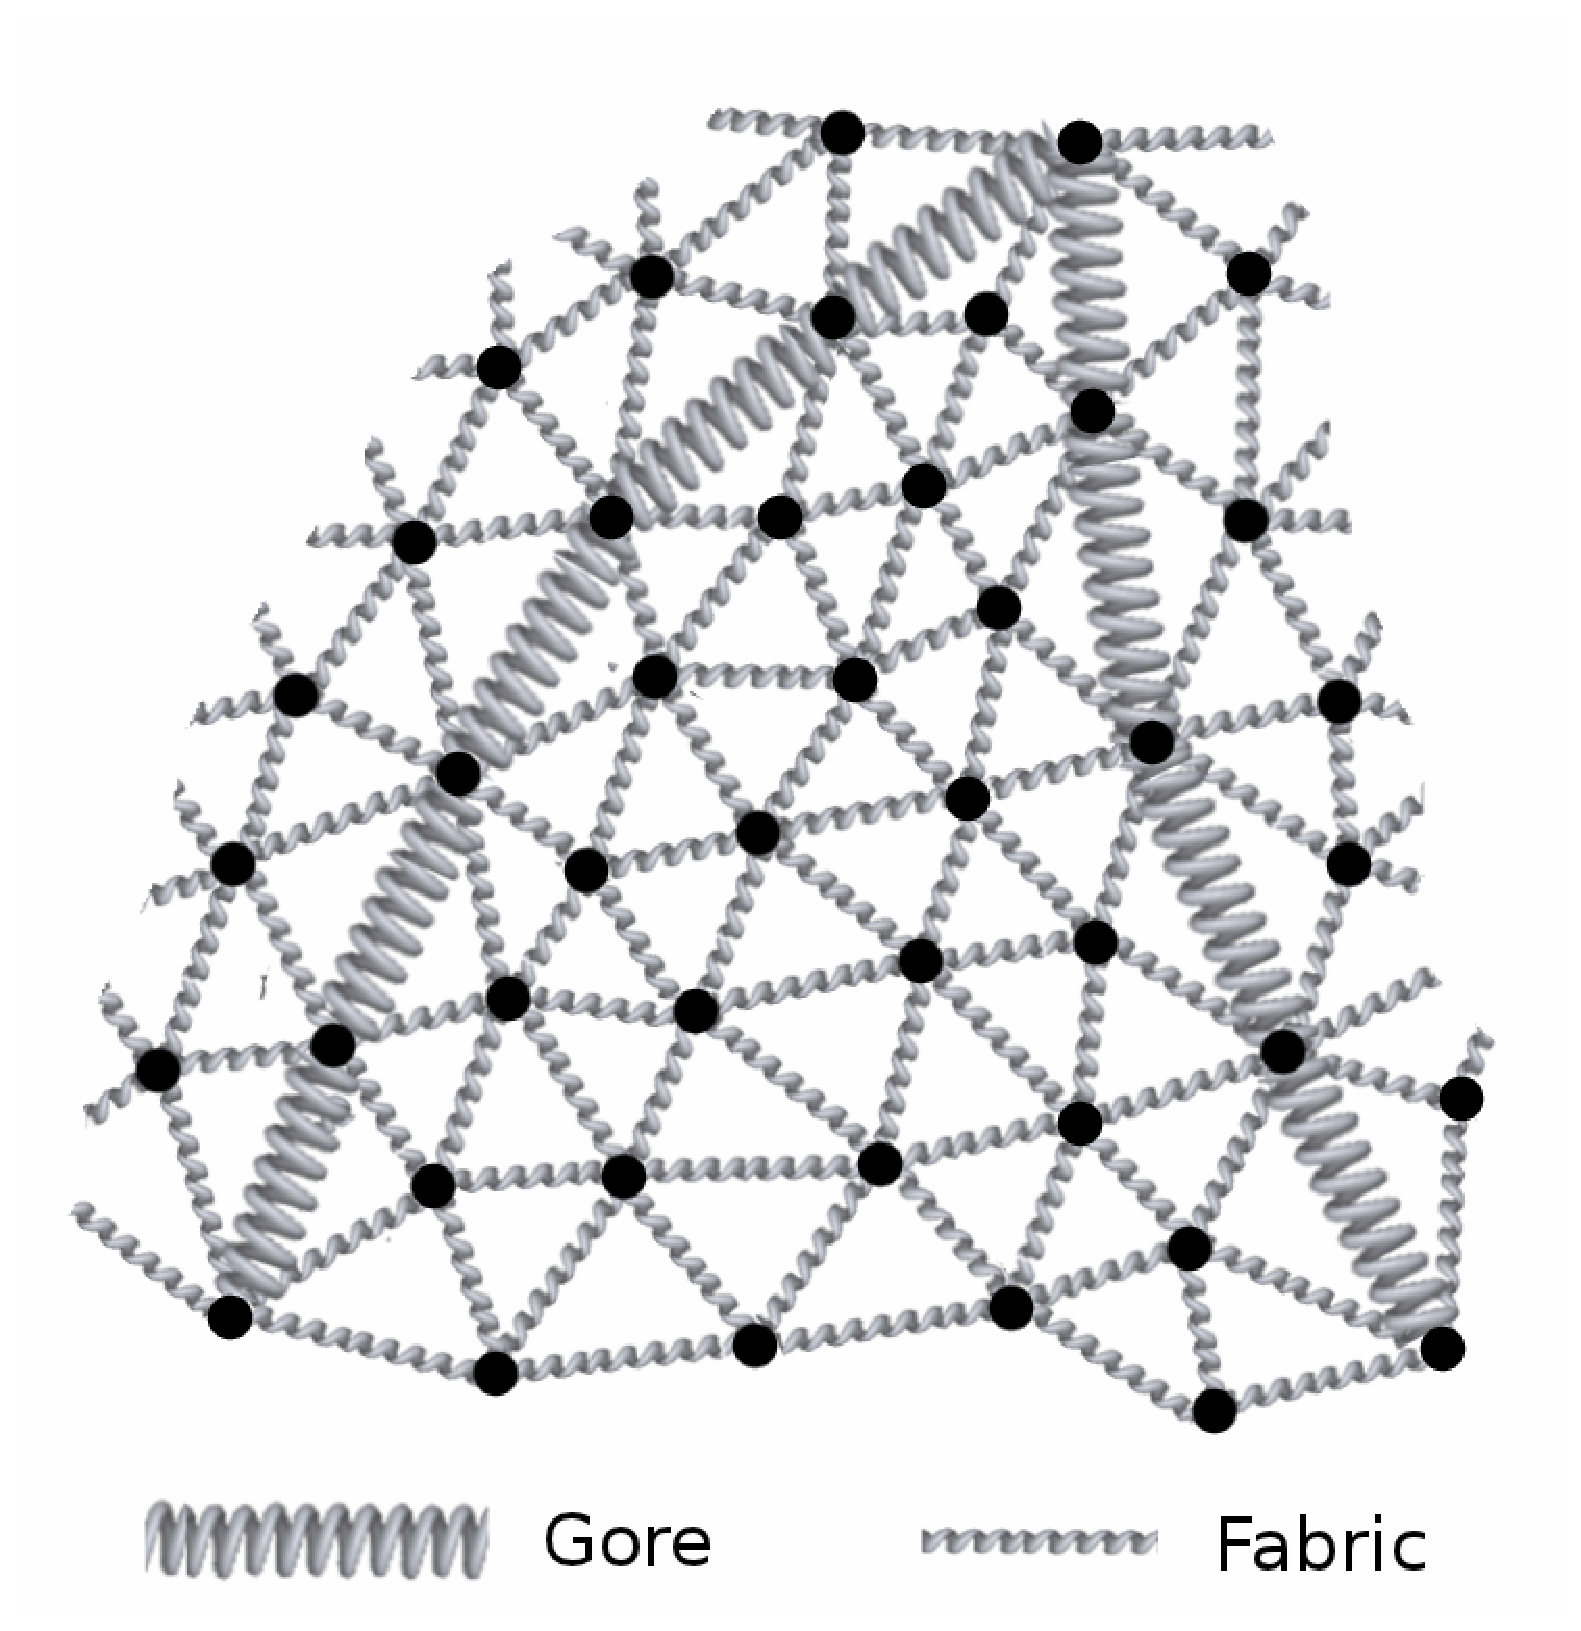
\epsfig{file=Figures/goremesh,width=0.55\hsize} \end{tabular} \caption{The
spring model on a triangulated mesh.} \label{fig:goremesh} \end{figure}

In order to interact with the environment, we also add external forces, such as gravity 
and air-drag, to the force term. The gravity force is a constant force, and thus easy to implement:
\begin{equation}
\vect{f}_{g,i} = m_i \vect{g}
\end{equation}
An accurate calculation of air-drag should include both the velocity shear (friction drag) and the stress (pressure drag) to the surface. However, since calculating the friction drag requires substantially more computational resources to resolve the boundary layer and its contribution to the drag force is minor in comparison with the pressure drag for the bluff body \cite{}, we have followed \cite{KalroTezduyar2000} to neglect the friction forces in the  current model, then the air-drag is formulated on a per-point basis:
\begin{equation}
\vect{f}_{p,i} = \sigma(p_i^- - p_i^+)\vect{n} \label{eq:drag}
\end{equation}
where $p_i^-$ and $p_i^+$ are the pressure of point $i$ on lower and upper sides of the canopy, $\sigma$ is the mass density of canopy per unit area, and $\vect{n}$ is the unit normal vector pointing from lower to upper side of the canopy. The pressure $p^-$ and $p^+$ are calculated by making use of the left state and right state of the interface point in the front tracking method.

Robust dynamic cloth simulation is critically dependent on well-chosen damping forces \cite{}. A strong damping force must be applied to the spring system with strong stretch force to prevent anomalous in-plane oscillations. However, this strong damping force should confine itself solely to damping in-plane motions without affecting other forces. In previous literatures \cite{}, the in-plane damping force for point $i$ is chosen as:
\begin{equation}
\vect{f}_{d,i} = -k_d m_i\sum_{j \neq i}(\vect{v}_i - \vect{v}_j)^T\vect{e}_{ij}\vect{e}_{ij}
\label{eq:damping_1} 
\end{equation}
It is tempting to formulate a damping function as above. However, this damping function only works for the case with fabric surface solely and gives nonsensical results for the case involving fabric connecting with strings. An alternative method is \cite{Terzopoulos87, Terzopoulos88, Carignan1992, Platt1988}'s treatment of cloth that used a simple viscous damping function which dissipated kinetic energy. We improve this method by subtracting the damping function with the external impulses, so that its influence on the external forces can be excluded:
\begin{equation}
\vect{f}_{d,i} = -k_d m_i(\vect{v}_i-I_{ext,i})
\end{equation}
where $I_{ext,i}(t,\vect{x}_i) = \int_0^t (\vect{f}_{g,i} + \vect{f}_{p,i}) dt$.
This method works well for all our cases including the joint fabric and strings, and produces visually appealing results. One problem of this method is that a linear function of velocity does not match the quartic energy functions of the continuum formulation \cite{Baraff1998}, but will put this as future studies in the new paper.

As discussed above, the fluid affects the motion of parachute canopy through the pressure drag and friction drag on the surface. In the opposite side, the parachute canopy is treated as an internal moving boundary for the fluid field. In this dissertation, the fluid field is modeled with incompressible Navier-Stokes equation, whose dynamics is controlled by the boundary conditions. The external boundary, such as inflow, outflow, periodic and wall boundaries can be handled trivially by defining an appropriate boundary condition following the underlying numerical scheme. As for the internal boundaries, the parachute canopy, we use the normal velocity computed from the ODEs of the spring system as the boundary value. Therefore, at each time step, we solve a Dirichlet boundary problem for the Naiver-Stokes equation.
\subsection{Porosity modeling}
Although the canopy surface can be modeled using a pure particle system, a canopy surface still has many unique properties differing with a group of particles. 
Due to the porous structure of a
fabric surface, a fraction of the free-stream flow can go through the canopy
surface and stabilize the descent of the parachute \cite{Johari05}. 
Meanwhile, this secondary flow reduces the drag force on the canopy. 
An intuitive way to study the porous medium via numerical method is to model the microstructure and solve the fluid equation at the pore level. However, to resolve the details of the porous layer would require an extremely 
refined computational grid. Due to limited computational resources, it 
is more practical to describe the average aerodynamic motion of the 
canopy surface using a mesoscale model. In the mesoscale model, the 
fabric surface can be treated as an interface immersed in the fluid.
The intractable complexities of the porous structures are then released by 
approximating it with an equivalent homogenized porosity.  
This simplification is reasonable since the parachute canopy thickness is
extremely small compared to its radius. In the past few years, 
several authors have attempted to study fabric permeability
under this simplification. Tazduyar et al. \cite{TezduyarSathe2007IJNMF} proposed a
homogenized porosity model based on the finite element method and applied it 
to the simulation of T-10 parachute. This method is then modified in \cite{Takizawa2012ACME}
to simulate the geometric porosity (gaps and slits in ring-sail parachute) by assigning a locally-varying homogenized porosity to the canopy surface. 
Kim and Peskin studied the influence of porosity on
parachute stability in two dimensions \cite{kim2006twodim}. They generalized
the immersed boundary method to handle the porous immersed boundary by 
coupling it with Darcy's law \cite{nield2013}.  Wang \cite{wang2006porous} simulated 
three-dimensional fluid-structure interaction with porous parachute canopy using the
LS-DYNA code in which the interface is approximated by a rigid and porous
internal boundary coupling with the force computed using the Ergun equation \cite{nield2013}. Although specific details vary, there is a deep commonality amongst all the approaches: the porosity effects are seen by the fluid mechanics computation through establishing a relationship between the pressure drop and the permeability velocity through the interface.

Through this section, we present an alternative approach which combines 
good accuracy for holding the Ergun's equation with a very simple and efficient 
computational procedure. The idea of our method is 
outlined as the following: The fluid dynamics is 
described by the incompressible Navier-Stokes equations and numerically 
solved by the projection method \cite{KimMoin85}, 
which is then coupled to the Ergun equation \cite{nield2013} by imposing a pressure drop boundary condition at the interface \cite{caiazzo2011}. Since the pressure is obtained 
through the Poisson equation by using the projection method at each time step, 
it is convenient to use the GFM technique similar to the work in 
\cite{fedkiw1999,kang2000boundary,liu2000boundary} to handle the 
discontinuity of the pressure at the fabric surface with the Poisson 
solver. Liu et al. \cite{liu2000boundary} used level set function to 
interpolate the interface position, whereas with the front tracking method 
the interface is explicitly tracked as a set of topologically linked marker points.

The fabric porosity is simulated with the pressure drop condition at the interface:
\begin{eqnarray} \label{jumpcond} {[p]}_{\Gamma} &=& \alpha
\mathbf{u}_\Gamma\cdot \mathbf{n} + \beta |\mathbf{u}_\Gamma\cdot \mathbf{n}|
\mathbf{u}_\Gamma\cdot \mathbf{n} \\
{[u]}_{\Gamma} &=& 0 \end{eqnarray}
where $[p]_{\Gamma}=p^+ - p^-$ is the
pressure drop across the interface $\Gamma$; $p^+$ and $p^-$ are the pressure in
$\Omega^+$ and $\Omega^-$ respectively; $\mathbf{n}$ is the local unit normal
vector at the interface; $\mathbf{u}_\Gamma$ is the relative velocity between
interface and fluid field at the interface location. For the two parameters in
\Eq{jumpcond}, $\alpha$ is the viscous porosity coefficient and $\beta$ presents
the inertial porosity coefficient. $\beta \neq 0$ is used in the case of
turbulent flow with high Reynolds number.  Note that the sign of the subdomains
is decided by the normal vector of surface triangles which points from
$\Omega^+$ to $\Omega^-$.  In our application of parachute simulation, the
interface is an open surface, which means that $\Omega^+$ and $\Omega^-$ are
connected. Therefore $\Omega^+$ and $\Omega^-$ is only a valid concept locally
for the immediate vicinity of the fabric surface.

The interaction between fluid and fabric surface structure is handled by the
impulse method \cite{KimLiLi12} on the \FronTierp platform. The jump condition
\Eq{jumpcond} is considered by coupling the GFM with the finite difference
scheme at the projection step. We use the pressure-Poisson version of
projection method because the jump condition can be applied directly to the
Poisson equation.

Consider the computational domain $[L_x,U_x]\times[L_y,U_y]\times[L_z,U_z]$
which is discretized into $N_x\times N_y\times N_z$ cells of size $\Delta
x\times\Delta y\times\Delta z$. Let $\mathbf{u}^n_{ijk}$ represent the
numerical solution of velocity field at grid node  $\mathbf{x}_{i,j,k} =
[L_x+(i+0.5)\Delta x,L_y+(j+0.5)\Delta y, L_z+(k+0.5)\Delta z]$ at time $t^n =
n\Delta t$ and an analogous definition holds for the pressure $p^n_{ijk}$ ($i =
0,1,2,...,N_x-1$, $j = 0,1,2,...,N_y-1$, $k = 0,1,2,...,N_z-1$). The standard
pressure-Poisson version of projection method consists of the following steps:

Step 1: Compute the tentative velocity
\begin{eqnarray}
\frac{\mathbf{u}^*-\mathbf{u}^n}{\Delta t}+
[(\mathbf{u}\cdot\nabla_h)\mathbf{u}]^{n+1/2}
=\frac{\mu}{2\rho}\Delta_h(\mathbf{u}^*+\mathbf{u}^n)\\ B(\mathbf{u}^*) = 0,
\end{eqnarray} here $B(\cdot) = 0$ is the boundary condition for $\mathbf{u}$,
$[(\mathbf{u}\cdot\nabla_h)\mathbf{u}]^{n+1/2}$ is computed by the WENO scheme
\cite{WENO96} for the advection equation from $t_{n-1}$ to $t_{n}$ and then
extrapolated to $t_{n+1/2}$ \cite{KimMoin85}.

Step 2: Projection step
\begin{equation} \frac{1}{\rho}\Delta_h p^{n+1/2} =
\nabla_h\cdot \mathbf{u}^*/\Delta t \label{proj} \end{equation}

Step 3: Update new velocity
\begin{equation} \mathbf{u}^{n+1} = \mathbf{u}^* -
\frac{\Delta t}{\rho}\nabla_h p^{n+1/2} \label{newvel} \end{equation}
where
\begin{eqnarray} \label{divU} \nabla_h\cdot u =
\frac{u_{i+1,j,k}-u_{i-1,j,k}}{2\Delta x} +
\frac{v_{i,j+1,k}-v_{i,j-1,k}}{2\Delta y} +
\frac{w_{i,j,k+1}-w_{i,j,k-1}}{2\Delta z}\\ \label{gradP} \nabla_h p =
[\frac{p_{i+1,j,k}-p_{i-1,j,k}}{2\Delta x},
\frac{p_{i,j+1,k}-p_{i,j-1,k}}{2\Delta y},
\frac{p_{i,j,k+1}-p_{i,j,k-1}}{2\Delta z}]\\    \label{lapP} 
\begin{aligned}
\Delta_h p = \frac{p_{i+1,j,k}+p_{i-1,j,k}-2p_{i,j,k}}{\Delta x^2} +
\frac{p_{i,j+1,k}+p_{i,j-1,k}-2p_{i,j,k}}{\Delta y^2} \\ \quad
+\frac{p_{i,j,k+1}+p_{i,j,k-1}-2p_{i,j,k}}{\Delta z^2} \end{aligned}
\end{eqnarray}

The pressure jump condition is implemented while discretizing the pressure
function. Since the derivative is not defined through the interface, therefore,
the method by Liu in \cite{liu2000boundary} for the variable coefficient
Poisson equation is used to discretize the Laplacian operator in \Eq{proj} and
the gradient operator in \Eq{newvel}.  Liu used level set function
\cite{osher1988fronts} to determine the sign of the domain. In the front
tracking framework, one can use the local normal vector to decide the sign of a
grid point in the computational domain since the interface is explicitly
represented by topologically connected marker points \cite{GliGroLi98}.  For
example in \Fig{grid}, when discretizing at grid point $p_a$ along the $x$
direction, the sign of this point is defined by the sign of $\Phi_a =
\mathbf{v}_a\cdot \mathbf{n}_{\Gamma}$.  Therefore, the sign of a grid point is
allowed to vary when discretizing along different directions.

\begin{figure}[] \centering
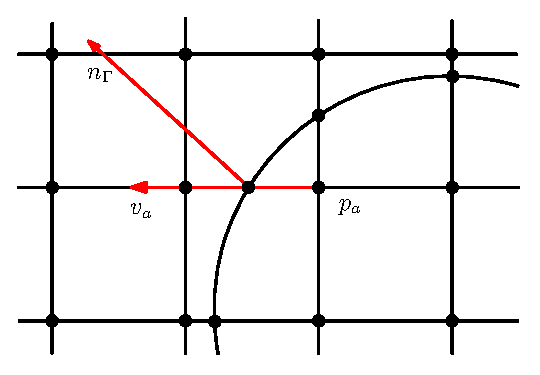
\includegraphics[width=0.6\textwidth]{Figures/grid.eps}
\caption{Numerical discretization near the interface. The plot
shows the algorithm for calculating
$\Phi_a = \mathbf{n}_\Gamma\cdot \mathbf{v}_a$, indicating the sign of the
domain at grid point $p_a$ when discretizing along $x$ direction. The normal
vector $\mathbf{n}_\Gamma$ at the interface-grid crossing is calculated by
\FronTierp with second order accuracy.}
\label{grid}
\end{figure}

Applying Liu's method to \Eq{proj} and \Eq{newvel}, we have
\begin{equation} \Delta_h p^{n+1/2}
= \nabla_h\cdot \mathbf{u}^*/\Delta t + F^x + F^y + F^z \label{newLap}
\end{equation} where $F^x = F^W + F^E$, $F^y = F^N + F^S$ and $F^z = F^T + F^B$.

\begin{equation} \label{newGrad} \mathbf{u}^{n+1} = \mathbf{u}^* - \Delta
t(\nabla_h p^{n+1/2} + G^x + G^y + G^z) \end{equation} where $G^x = G^W + G^E$,
$G^y = G^N + G^S$ and $G^z = G^T + G^B$.

The underlying idea to derive the additional terms in \Eq{newLap} and
\Eq{newGrad} is to define a ghost value for each grid node by imposing the jump
condition
\begin{equation} p_{i,j,k}^+ - p_{i,j,k}^- = a(\mathbf{x}_{\Gamma})
\label{disJump} \end{equation} where the indices "$\pm$" stand for the domain as
$\Omega^{\pm}$ and $a(\mathbf{x}_{\Gamma})$ is the pressure drop at the
interface location $\mathbf{x}_{\Gamma}$.  In consequence, every grid node has
two values for the solution, the real value and the ghost value.

According to the GFM, all the variables in the difference equation discretized
at point $\mathbf{x}_{i,j,k}$ should use the same domain indices as $\mathbf{x}_{i,j,k}$.
For example, if $\mathbf{x}_{i,j,k}$ is in domain of $\Omega^+$, then \Eq{gradP} becomes

\begin{equation} \label{ghostGradP} \nabla_h p =
[\frac{p^+_{i+1,j,k}-p^+_{i-1,j,k}}{2\Delta x},
\frac{p^+_{i,j+1,k}-p^+_{i,j-1,k}}{2\Delta y},
\frac{p^+_{i,j,k+1}-p^+_{i,j,k-1}}{2\Delta z}] \end{equation} and \Eq{lapP}
becomes
\begin{equation} \label{ghostLapP} 
\begin{aligned} \Delta_h p =
\frac{p^+_{i+1,j,k}+p^+_{i-1,j,k}-2p^+_{i,j,k}}{\Delta x^2} +
\frac{p^+_{i,j+1,k}+p^+_{i,j-1,k}-2p^+_{i,j,k}}{\Delta y^2} \\ \quad
+\frac{p^+_{i,j,k+1}+p^+_{i,j,k-1}-2p^+_{i,j,k}}{\Delta z^2} \end{aligned}
\end{equation}
In the case of $\Phi_{i,j,k} \cdot \Phi_{i+1,j,k} < 0$, that is
$\mathbf{x}_{i+1,j,k}$ is in the different domain from $\mathbf{x}_{i,j,k}$,
the ghost value $p^+_{i+1,j,k}$ should be replaced by its real value using the
jump condition \Eq{disJump}. It is easy to obtain
$F^E = -a(x_{\Gamma})/(\Delta x^2)$ and $G^E = -a(\mathbf{x}_{\Gamma})/(2\Delta x)$.

In the case of $\Phi_{i,j,k}\cdot\Phi_{i+1,j,k} > 0$, that is no interface exists between point $\mathbf{x}_{i,j,k}$ and $\mathbf{x}_{i+1,j,k}$, then $F^E = G^E = 0$.  The derivation of other terms is ignored here, since they are a straightforward extension of the above procedure.

In our situation, $a(\mathbf{x}_{\Gamma}) = [p]^n_{\Gamma} = \alpha
\mathbf{u}_{\Gamma}^n\cdot \mathbf{n} + \beta|\mathbf{u}_{\Gamma}^n\cdot
\mathbf{n}| \mathbf{u}_{\Gamma}^n\cdot \mathbf{n}$, where $\mathbf{u}_{\Gamma} =
\mathbf{u}_{interface} - \mathbf{u}_{fluid}$, $\mathbf{u}_{interface}$ is the
velocity of the interface point and $\mathbf{u}_{fluid}$ is obtained by using
the bilinear interpolation of the velocity field at the interface location.

\subsection{Collision handling}
Resolution of collision between different parts of
fabric surface or between fabric surface and environment is a very delicate
problem in mathematical algorithm and computational geometry. Since all points 
are on the surface and all points may collide with each other, collision has been 
a major bottleneck in cloth simulation. In order to resolve fabric collision during parachute inflation process or its reverse procedure (parachute folding), we have followed the algorithm proposed by \cite{Bridson02} and implemented a collision handling function to detect and unwrap the fabric surface in each time step. Comparing with other previous methods, such as \cite{Provot1997, Volino1995}, which allow self-interference and recover from it later, this approach is based on repulsion forces and non-stiff penalty forces. It can guarantee no dynamic self-interference of cloth, and thus do not need complicated and unreliable algorithms for detecting and fixing self-intersection. Furthermore, this method is able to produce physically plausible details, such as bulk and small scale crumpling, by considering the friction forces.

Our approach for collision detection/response is similar to \cite{Bridson02}, but with some key differences in the implementation. Since in the parachute simulation, various types of materials are involved in the collision, such as parachute canopy, suspension lines and rigid cargoes, a unified collision framework is required to handle their interactions. 
 
The basic procedure of the algorithm is as follows:
\begin{itemize}
\item Select a collision time step size $\Delta t$ and set $t^{n+1}=t^{n}+\Delta t$
\item Record positions $\mathbf{x}^n$ of mass points at $t^n$
\item Compute spring mesh interior dynamics to get candidate positions
$\bar{\mathbf{x}}^{n+1}$
\item Calculate average velocity with
$\bar{\mathbf{v}}^{n+1/2} = (\bar{\mathbf{x}}^{n+1}-\mathbf{x}^n)/\Delta t$
\item Call collision solver to modify $\bar{\mathbf{v}}^{n+1/2}$ to avoid any interferences and obtain the final mid-step velocity $\mathbf{v}^{n+1/2}$
\item Compute the final position
$\mathbf{x}^{n+1} = \mathbf{x}^n+\mathbf{v}^{n+1/2}\Delta t$
\item Advance the mid-step velocity $\mathbf{v}^{n+1/2}$ to $\mathbf{v}^{n+1}$ \end{itemize}

We will focus on the step of collision resolution since other steps are trivial. As in \cite{Bridson02}, the collision detection and response consist of a few subroutines: proximity detection, collision detection and fail-safe method. For efficient proximity detection, an axis aligned bounding boxes hierarchy (AABB tree) is built bottom-up at the beginning of the simulation and will be recalculated for each iteration of the collision algorithm. The bounding boxes are created by taking a box around each geometric element enlarged by the thickness of the cloth. In the parachute simulation, two types of elements need to be considered: triangle for parachute canopy and bond for suspension lines. After creating the AABB tree, we can efficiently traverse the potential collision by only considering the geometric elements with intersected bounding boxes. It is obvious that the potential collisions drop into three categories: triangle to triangle, triangle to bond , and bond to bond. These cases can be further simplified into the cases of "edge to edge" and "point to triangle". Note that we don't check a point against a triangle that contains it or two edges shares an endpoint. If the distance between a point and a triangle or two edges is smaller than the fabric thickness, a repulsion force is applied to the two elements to stop the proximity and a non-stiff penalty force is also used to prevent the collisions in the future. The second subroutine, collision detection, is similar to the proximity detection, except that the bounding boxes are enlarged to contain both the old state and the current state. This helps to detect the intersection between the moving trajectories of two elements. When a real collision occurs, the corresponding two elements are rewound back to the exact moment of collision and applied with the repulsion forces. Finally, the fail-safe method, impact zone method, is necessary since the collision handling procedure follows the iteration methodology and it is not guaranteed to terminate in finite number of steps. This is mainly because resolving old collision may bring new collision to the surface. As stated in \cite{}, the principle of the impact zone method is to combine all the points in collision to form a large rigid surface. The points in the rigid surface have no relative motion, and hence all collisions can be quickly eliminated. However, this impact zone method has a tendency to freeze the cloth into nonphysical clumps. Therefore, we only switch to the impact zone method after a few iterations to quickly eliminate all collisions.

It is known that the parachute inflations process includes the interactions of rigid bodies (cargo, parachutist), elastic surfaces (parachute canopy) and elastic curves (suspension line). The combination gives six unique situations and make the algorithm not easy to implement. In the programming design of point view, our solution to this problem is to use an abstract C++ class to represent the collision elements: both the "bond" and "triangle". This abstract class provides interface to give their minimum and maximum coordinates in each direction, as well as iterators for all the points in the element. By doing this, the collision algorithm works without knowing the element is a triangle or a line segment. As for the rigid body, we merge all the rigid points to form a large impact zone before the collision detection and handling. Since the impact zone method essentially duplicates the motion of a rigid body, the remaining collision procedure does not need to be changed at all. 

There are many ways to construct the impact zone. Our implementation uses the famous "union and find" algorithm \cite{}. Before the collision algorithm starts, each point is in its own list. Then, when a point-triangle or edge-edge collision occurs, the lists containing the four points are merged together into one larger impact zone. The impact zones are grown until the cloth is collision free. The velocity of the points in the impact zone is derived from a rigid body motion that preserves linear and angular momentum.

In summary, this method can guarantee no dynamic self-interference of cloth after a successful call of the function. We coupled our collision handling function with the {\it
FronTier++} library, and utilized OpenMP to parallelize the traverse of the triangle
list. Our algorithm can universally handle various collision situations between rigid bodies, fabrics and strings. \Fig{fig:collision} shows the numerical results of the six collision situations.

\subsection{Parallelism} 
The \FronTierp library offers functions for parallelized
operations of initialization and front propagation. On parallel platform, the
computational domain is divided into a partition of dimensions. A buffer
interface is attached at the boundary of each subdomain. After propagation of
the interface in each time step, the buffer surface is updated through exchange
of interface geometry and state data with the neighboring subdomains. For
parachute simulation, we use PETSc to solve for the Navier-Stokes equation in
both the advection and projection steps.  The parallelization of ODE solver for
the parachute canopy is more challenging.  It is parallelized through the OpenMP
or the GPU platform.

\begin{figure}[!ht] \centering \begin{tabular}{ccc}
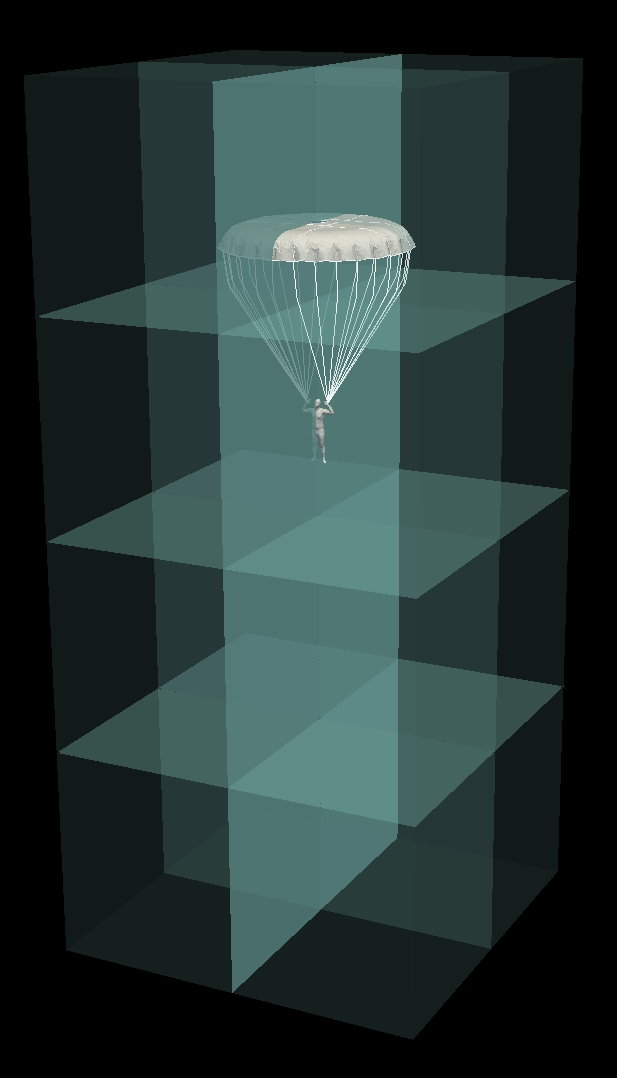
\epsfig{file=Figures/parallel-16-0,width=0.25\hsize}
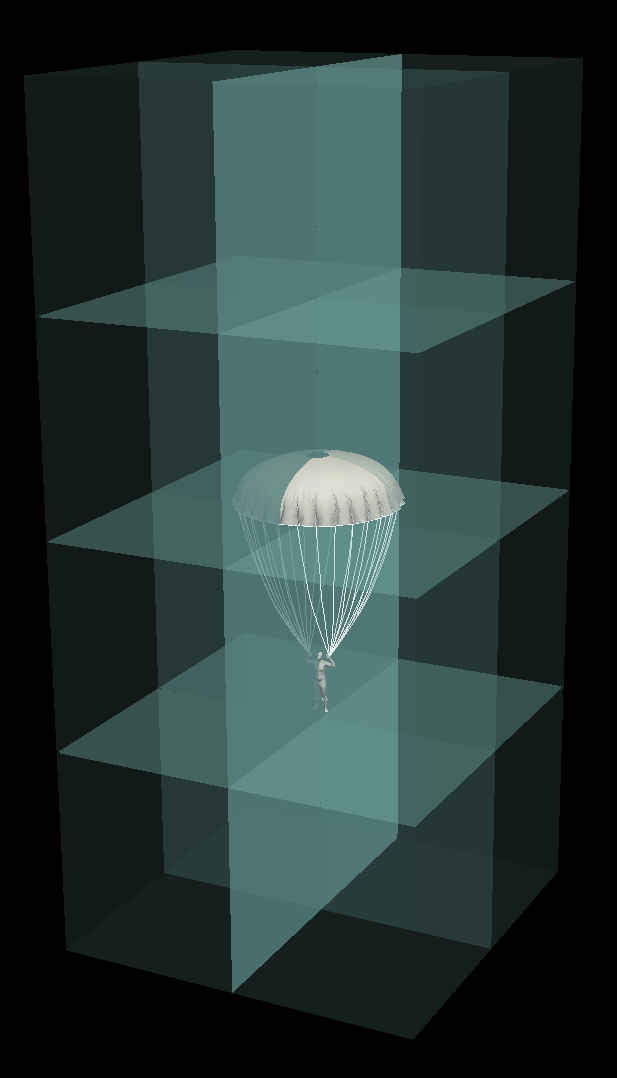
\epsfig{file=Figures/parallel-16-1,width=0.25\hsize}
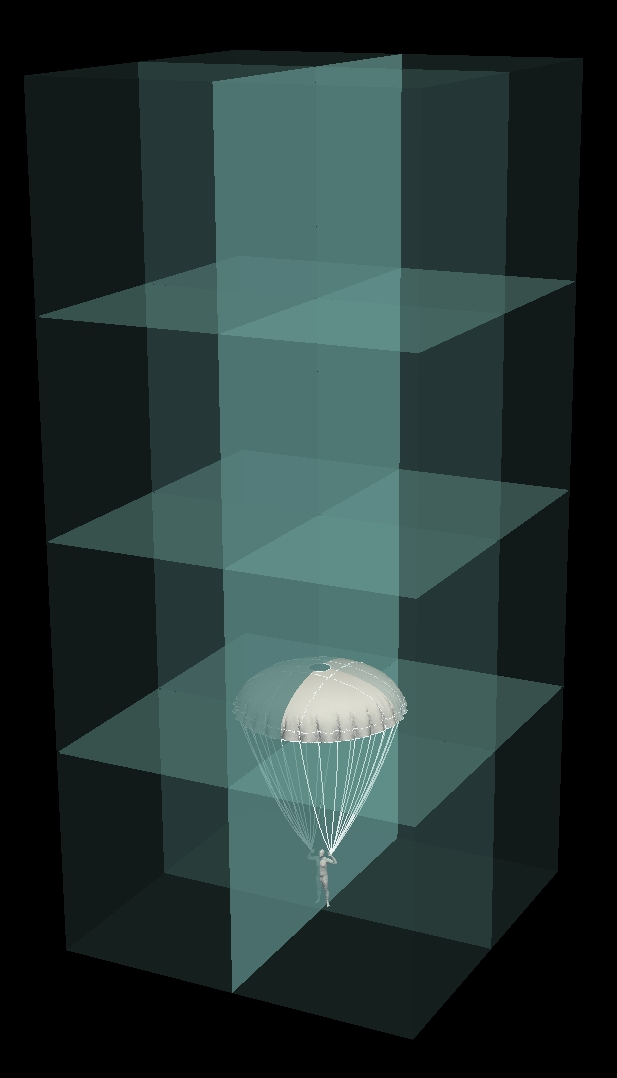
\epsfig{file=Figures/parallel-16-2,width=0.25\hsize} \end{tabular} \caption{
Parallel simulation of parachute descending on Dell Precision T7600 Workstation
with 16 subdomains. The neighboring subdomains are communicated via MPI while
the spring model is solved on OpenMP or GPU system.  The numerical algorithm is
capable of running on parallel computer with many processors but requires tuning
for efficiency and load balance.  \label{fig:parallel}} \end{figure}

Graphics Processing Unit (GPU) computing \cite{kirk2010programming} is to use
the GPUs together with CPUs to accelerate a general-purpose scientific and
engineering application.  GPU computing can offer dramatically enhanced
application performance by offloading computation-intensive portions of the
programming code to the GPU units, while the remainder of the code still runs on
the CPU.  Joint CPU/GPU applications constitute a powerful combination because
CPUs consist of a few cores optimized for serial processing, while GPUs consist
of thousands of smaller, more efficient cores designed for massive parallel
calculations.  Serial portions of the code with logical comparison run on the
CPU while floating point operation intensive parallel portions of the code run
on the GPU.

Our current strategy is to collect the point data to a sever processor and then
apply OpenMP or GPU solver in each of the sever nodes. This algorithm is not
efficient and does not scale linearly as the total number processors is
increased. We are testing several different alternatives and comparing pros and
cons of each method.

Global indexing is a new feature added to the \FronTierp computational library
for fluid structure interaction.  Since the original \FronTierp
\cite{DuFixGli05} deals with frequent surface mesh optimization and topological
reconstruction, its parallelization is based on the floating point matching.
The floating point matching is not completely reliable therefore more
complicated algorithms were implemented as the reinforcement.  For fabric-like
surface, especially when a spring-mass model is used, the inter-connectivity and
proximity of the interface marker points are static. Therefore, global indexing
is ideal for the parallel communication of the surface information and is now
employed in the work.  This new feature enables the parallel communication of
interface topology and geometry on a much more reliable and robust basis. It has
greatly reduced the run-time interruption due to bugs and efficiency in
geometrical and topological matching.

\section{Numerical study of turbulent entrainment and mixing processes}
Another application of the current computing framework is the numerical study 
of turbulent entrainment and mixing processes at the boundary of a cloud. During the entrainment and mixing process, large eddies driven by the convective circulation engulf large volumes of environmental air deep into the cloud core. As turbulent mixing develops, these volumes are stretched and compressed into thinner filaments until the Kolmogorov scale is reached, where final homogenization occurs through the molecular diffusion process \cite{Burnet2007Observational}. Through entrainment and mixing with environment, the cloud water is diluted and transported by turbulence. In the previous bulk cloud models \cite{Grabowski1990}, the thermodynamic grid-averaged equations are used to describe the potential temperature, water vapor and cloud water mixing ratios. These model distinguish the evaporation and condensation scenarios according to the grid-averaged thermodynamic fields, and artificially adjust the grid box back to saturation as long as there is enough cloud water in the case of evaporation. This adjustment is based on the assumption that the vapor field in the subgrid cell is uniformly distributed during one time step. However, when the subgrid-scale structures of the thermodynamic fields exist, it is possible that the grid-averaged fields imply conditions below saturation and some cloud water does exist. Such conditions can occur, for instance, a part of the box is saturated and contains some cloud water, and the other part remains unsaturated and cloud-free \cite{Grabowski2007}. In many literatures\cite{Baker1980, Burnet2007, Lehmann2009}, two extreme cases are usually used to describe the mixing processes: extremely homogeneous mixing and extremely inhomogeneous mixing. In the extremely homogeneous case, the mixing process is so fast that all the cloud droplets stay in the same environment, and yet in the extremely inhomogeneous scenario, a part of the droplets completely disappear before others begin to evaporate. In consequence, the homogeneous mixing only changes the averaged droplets size before completely evaporation happens, while the inhomogeneous mixing remains the mean droplets size with a decreasing number density.

The entrainment and mixing process is important for the evolution of a cloud, but until now it was poorly understood that whether the reduction of liquid water content during entrainment was through the reduction of only the droplet size (extremely homogeneous mixing), or only the number of droplets (extremely inhomogeneous mixing), or both the number and size (inhomogeneous mixing). These situations can be quantified by comparing two time scales: the turbulent homogenization time scale and thermodynamic time scale associated with the evaporation process. In the extreme cases, one time scale will dominate the other, otherwise the two scales are comparable. Recently, it has been demonstrated that different mixing scenarios can occur and change during one single cloud evolution (\cite{And09,Burnet07,Lehmann09}) and therefore it becomes more and more important to have a reasonable and accurate estimation of the mixing scenario for a subgrid model. \cite{Jarecka2013}, utilized the DNS results from \cite{And04,And06,And09}  to estimate the mixing scenario with a parameter $\alpha$ and merged the $\lambda$-$\beta$ subgrid scheme (\cite{Jarecka2009}) with the double-moment LES model(\cite{Morrison2008}). \cite{Lu2013}, proposed the transition scale number to measure the occurrence probability of homogeneous or inhomogeneous entrainment-mixing process (homogeneous mixing degree). Both the cloud observations and numerical simulations imply a positive relationship between the transition scale number and the homogeneous mixing degree. In spite of many progresses in the study of cloud microphysics, to capture the details of turbulent transportation and dilution of cloud water remains a challenge for representing clouds in coarse-resolution climate model.

In this section, we describe a new particle-resolved three dimensional direct numerical simulation (DNS) model that combines Lagrangian droplet tracking with the Eulerian field representation. The new model consists of the turbulence environment, scalar fields and particle system, and thus can be easily built under the computational framework proposed in this paper.

\subsection{Model Description}
Similar to most previous DNS, our new DNS is based on the incompressible
Boussinesq fluid system \cite{And04}. Briefly, the temperature $T$ and vapor
mixing ratio $q_v$ are described by the following equations \cite{Kumar11}:

\begin{equation}
\partial_{t}T+(\mathbf{u}\cdot\nabla)T=\frac{L_{h}}{c_{p}}C_{d}+\mu_{T}\nabla^{2}T\label{eq:Temp}
\end{equation}

\begin{equation}
\partial_{t}q_{v}+(\mathbf{u}\cdot\nabla)q_{v}=-C_{d}+\mu_{v}\nabla^{2}q_{v}\label{eq:Vapor}
\end{equation}

where $L_{h}$ is the latent heat of water vapor condensation,
$c_{p}$ is the specific heat at constant pressure, $\mu_{T}=\mu_{v}$ are
the molecular diffusivity for temperature and water vapor, respectively
and assumes to be equal. The condensation rate $C_{d}$ denotes the rate of exchange between liquid and vapor, and is described by:

\begin{subequations}

\begin{equation}
C_{d}(\mathbf{X},t)=\frac{d(m_{l}(\mathbf{X},t))}{m_{a}dt}=\frac{4\pi\rho_{l}K}{\rho_{0}a^{3}}\Sigma_{i=1}^{n}S(\mathbf{X}_{i},t)R_{i}(t)\label{eq:CondRate}
\end{equation}


where $K$ is a function of temperature and pressure given by:

\begin{equation}
K=1/[(\frac{L_{h}}{R_{v}T}-1)\frac{L_{h}\rho_{l}}{C_{T}T}+\frac{\rho_{l}R_{v}T}{De_{s}(T)}]\label{eq:CondCoeff}
\end{equation}


where $R_{v}$ is the individual gas constant, 
$C_{T}$ is the coefficient of thermal conductivity, $e_{s}(T)$ is
the saturation vapor pressure. The supersaturation $S(X,t)$ is calculated
directly from the water vapor mixing ratio and temperature from the following
equation

\begin{equation}
S(\mathbf{X},t)=\frac{q_{v}(\mathbf{X},t)}{q_{v,s}(\mathbf{X},t)}-1\label{eq:Supersat}
\end{equation}

\end{subequations}

where $q_{v,s}$ is the corresponding saturated water vapor mixing ratio. The droplets
will grow or shrink depending on the sign of supersaturation $S$.

The liquid water mixing ratio is given by
\begin{equation}
q_{c}(\mathbf{X},t)=\frac{4\pi\rho_{l}}{3\rho_{0}a^{3}}\sum_{i=1}^{n}R_{i}^{3}(t)\label{eq:cloud_water}
\end{equation}


where $a$ is the size of a grid cell, $n$ is the number of droplets
in the grid cell; $\rho_{l}$ and $\rho_{0}$ are the densities of water
and air. $R_{i}(t)$ is the radius of the $i$-th droplet.

The dynamical field is given by
\begin{subequations}

\begin{equation}
\partial_{t}\mathbf{u}+(\mathbf{u}\cdot\nabla)\mathbf{u}=-\frac{1}{\rho_{0}}\nabla p+\nu\nabla^2 \mathbf{u}+\mathbf{f}_b + \mathbf{f}_e\label{eq:NS1}
\end{equation}


\begin{equation}
\nabla\cdot \mathbf{u}=0\label{eq:NS2}
\end{equation}

\end{subequations}

where $\nu$ is the kinetic viscosity, $\rho_{0}$ is the density of
dry air, $\mathbf{u}$ is the velocity field, $p$ is the pressure field. Here $\mathbf{f}_b$ is the force immitating the buoyancy effects:
\begin{equation}
\mathbf{f}_b= 
-\mathbf{g}[\frac{T-T_{0}}{T_0}+0.608(q_{v}-q_{v0})-q_{c}]
\label{eq:source_term}
\end{equation}
where $\mathbf{g}$ is the gravity, $T$ and $q_{v}$ are temperature
and vapor mixing ratio field respectively with the subscript ``$0$''
denoting the reference value. $\mathbf{f}_e$ is the artificial external force defined in the Fourier space.

To describe the motion and condensation(or evaporation) of cloud droplets, we use

\begin{equation}
R(t)\frac{R(t)}{dt}=K\cdot S(\mathbf{X},t)\label{eq:Radius}
\end{equation}


\begin{equation}
\frac{d\mathbf{X}(t)}{dt}=\mathbf{V}(t)\label{eq:Coords}
\end{equation}


\begin{equation}
\frac{d\mathbf{V}(t)}{dt}=\frac{1}{\tau_{p}}[\mathbf{u}(\mathbf{X},t)-\mathbf{V}(t)]+\mathbf{g}\label{eq:Velocity}
\end{equation}

Here $R(t)$ is the radius, $\mathbf{X}(t)$ is the position coordinate and
$\mathbf{V}(t)$ is the droplet velocity, $\mathbf{g}$ is the gravitational
constant. $\tau_{p}=2\rho_{l}R^{2}/(9\rho_{0}\nu)$ is the finite particle
response time. The particle response time measures the droplet inertial
effects; when $\tau_{p}$ is set to be zero, equation (\ref{eq:Velocity})
becomes $\mathbf{V}(t)=\mathbf{u}(\mathbf{X},t)$, which implies that the
droplets will exactly follows the turbulent flows. The last term in equation
(\ref{eq:Velocity}) is the sedimentation term that accounts for the effect of
gravity on droplets motion. Equation (\ref{eq:Velocity}) is appropriate if the
Reynolds number based on the relative velocity between the particle and fluid
is significantly less than one \cite{Eaton94}. The particle diameter is also
assumed to be smaller than the Kolmogorov microscale $\eta$, the smallest
length scales of the turbulent flow field. During condensation, direct
interactions between droplets are negligible because their sizes are too small
comparing with the average distance between two droplets.

The dynamic equations \Eq{eq:NS1} and \Eq{eq:NS2} are solved following the
fraction-step algorithm \cite{Brown2001}. The thermodynamic fields
\Eq{eq:Temp}, \Eq{eq:Vapor} are solved with semi-implicit method coupling with
fifth-order WENO scheme for the discretization of the hyperbolic term. The use
of WENO scheme here is critical since it can well handle the numerical
overshoots as well as keep the high order of the overall accuracy. To simplify
the implementation, we adopt the external package PETSc \cite{petsc_cite} as
the parallel linear solver and HYPRE \cite{hypre_cite} as the high performance
preconditioner. These two packages are widely used in the community of
computational fluid dynamics and has a good parallel scaling in both Linux
cluster and supercomputer.The Droplets position (\Eq{eq:Coords}) and motion
(\Eq{eq:Velocity}) are solved by implicit Euler method in consideration of
efficiency and stability. The time step size is adaptive to satisfy the
Courant-–Friedrichs-–Lewy (CFL) condition. Parallel computing techniques are
implemented with MPI library to increase the computational speed.

\subsection{Initial turbulence field and external forcing}
Since the DNS is performed in a small-scale turbulence environment, it is necessary to generate and maintain a physical turbulence field before injecting the particles into it. Many literatures \cite{} have demonstrated that the small-scale behavior in turbulent flows tends to be characterized by statistical homogeneity, isotropy and universality. Because of the universality we can hope to understand small-scale behavior by studying the simplest turbulent flows: homogeneous, isotropic turbulence. The two most frequently studied types of isotropic turbulence are freely decaying, and forced statistically stationary turbulence, which are both studied in this dissertations. The decaying turbulence can be easily obtained by providing a solenoidal isotropic initial velocity field with random phases and prescribed energy spectrum, and then directly solve the Navier-Stokes equation to evolve the turbulence. In addition to the initial condition, the forced turbulence further requires a method to artificially force the low-wavenumber modes, so as to supply the energy dissipated by viscous effects. The energy-containing motions are, therefore, unnatural and are not governed by the Navier-Stokes equations. However, insofar as the small-scale motions are universal, useful information about them can be extracted provided that there is wide separation between the largest and smallest scales. The initialization and external forcing method for homogeneous, isotropic turbulence are introduced below. 

Similar to Rogallo's procedure, the initial velocity field is constructed in Fourier space satisfying continuity, isotropy, and having a given energy spectrum. Given the coordinates in three-dimensional Fourier space $\vect{k} = \{k_1, k_2, k_3\}$ and energy spectrum $E(k)$, the Fourier transformation $\hat{\vect{u}}$ of the velocity field is determined by:
\begin{equation}
\hat{\vect{u}} = \left\{\frac{\alpha kk_2 + \beta k_1k_3}{k(k_1^2 + k_2^2)^{1/2}},
\frac{\beta k_2k_3 - \alpha k k_1}{k(k_1^2 + k_2^2)^{1/2}}, 
- \frac{\beta (k_1^2 + k_2^2)^{1/2}}{k}\right\}
\end{equation}
where $k = (k_1^2 + k_2^2 + k_3^2)^{1/2}$. The coefficients $\alpha$ and $\beta$ are 
\begin{equation}
\alpha = (\frac{E(k)}{4\pi k^2})^{1/2}e^{i\theta_1}\cos{\phi},\quad
\beta = (\frac{E(k)}{4\pi k^2})^{1/2}e^{i\theta_2}\sin{\phi}
\end{equation}
where $\theta_1$, $\theta_2$, and $\phi$ are uniformly distributed random numbers on the interval $(0, 2\pi)$. It can be verified that $\hat{\vect{u}}$ satisfies the continuity condition $\hat{\vect{u}}\cdot\vect{k} = 0$
The energy function is defined as:
\begin{equation}
E(k) = \frac{16}{\sqrt{\pi/2}}\frac{u^2_{rms}k^4}{k_0^5}\exp(-\frac{2k^2}{k_0^2})
\end{equation}
where $u_{rms}$ is the initial root-mean-square (r.m.s) velocity, and $k_0$ is the wavenumber at which the maximum of $E(k)$ occurs. The parameters $u_0$ and $k_0$ determine
the exact power spectral shape. Different from the commonly used Kolmogorov
spectrum, this function enforces the kinetic energy be concentrated in a
relatively narrow band at the initial time, so as to not affect the turbulence
behavior in larger wave number space. As turbulence evolves, the spectrum will
quickly spread to the inertial range and dissipation range according to the
Navier-Stokes equation. \Fig{fig:eng_spr} illustrates the energy spectrum with
different parameters. The parameters for most cases in this paper are $u_0 =
0.35m/s$ and $k_0 = |(1,1,2)| \approx 2.4$, which allows one to generate an
initial turbulence field with reasonable Reynolds number and narrow energy band
in large wave length.

\begin{figure}\centering
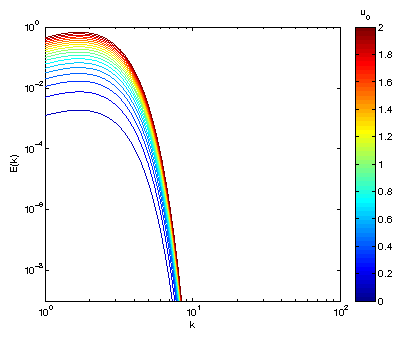
\includegraphics[width=0.48\textwidth]{Figures/eng_spr_u}
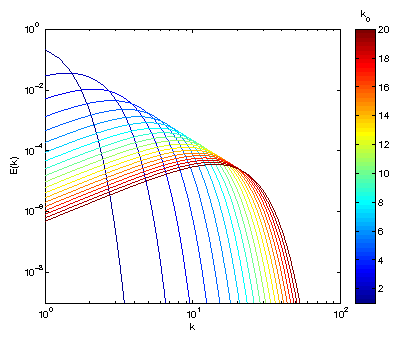
\includegraphics[width=0.48\textwidth]{Figures/eng_spr_k}
\caption{Initial energy spectrum with different parameters: left figure shows the energy spectrum with fixed $k_0 = 2.4$ while varing $u_0$ from $0m/s$ to $2m/s$, right figure shows the one with fixed $u_0 = 0.35m/s$ and varing $k$ from $1$ to $20$.\label{fig:eng_spr}}
\end{figure}

As for the external volume force, several solutions have been proposed in the literature, representing two main approaches. The first is to construct the force in Fourier space to keep a constant energy injection rate, and thus this method requires knowledge of Fourier-transformed velocities. In \cite{Ghosal1995Dynamic, Carati1995Representation}, the authors applied a force to the wavenumbers in the chosen shell, and guarantee a constant energy injection rate. The Ghosal's approach can be simply formulated in the Fourier space: 
\begin{equation}
\mathbf{f}_e(\mathbf{k},t) = \epsilon_{in}\frac{\mathbf{u}(\mathbf{k},t)}
{\sum_{\mathbf{k}_f\in \kappa}|\mathbf{u}(\mathbf{k}_f,t)|^2}
\sigma_{\mathbf{k},\mathbf{k}_f}
\end{equation}
where $\mathbf{u}(\mathbf{k},t)$ is the Fourier-transformed velocity function, $\mathbf{k}_f$ is chosen from a subset of the wavenumber space $\kappa$ containing a few wavevectors, for example $(1,1,2)$ plus all permutations with respect to components and sign, $\epsilon_{in}$ is a constant input energy rate. $\delta_{k,k_f}$ is a delta function. Therefore, statistics stationary homogeneous turbulence can be obtained in DNS by forcing the low-wavenumber modes. There still exist many other approaches based on the Fourier transformation. For example, Sullivan and Chasnov attempted to maintaining constant kinetic energy in the lowest wavenumbers \cite{Sullivan1994Deterministic, Chasnov1991Simulation}. Eswaran and Pope in \cite{Pope1988Examination} utilized a stochastic process to determine external forcing scheme. 

The second group is to evaluate the external force in physical space. This approach is attractive for applications since it does not require transformation to Fourier space and is easily integrated into physical-space numerical codes. Lundgren proposed a forcing function which is directly proportional to the velocity \cite{Lundgren2003Linearly}. Rosales studied the properties of this linear forcing scheme for isotropic turbulence, and showed the linearly forced system converges to a stationary state that does not depend on the spectral shape of the initial condition \cite{Rosales2005Linear}. The Lundgren's linear forcing scheme is determined with the following equation:
\begin{equation}
\vect{f}(\vect{x}, t) = \frac{\epsilon_{in}}{3u_{rms}^2}\vect{u}
\end{equation}
During the simulation, the root-mean-square velocity $u_{rms}$ is recalculated every time step while the energy injection rate $\epsilon_{in}$ is kept equal to a constant.
The cross section of the initial and stationary vorticity field is displayed in \Fig{vort}.

\begin{figure}[h]\centering
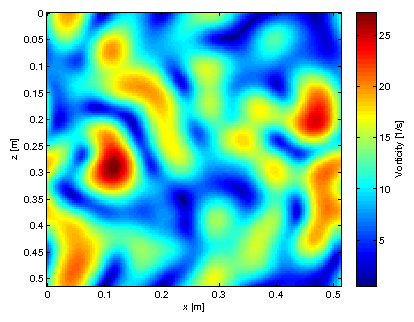
\includegraphics[width=0.48\textwidth]{Figures/vortex-0}
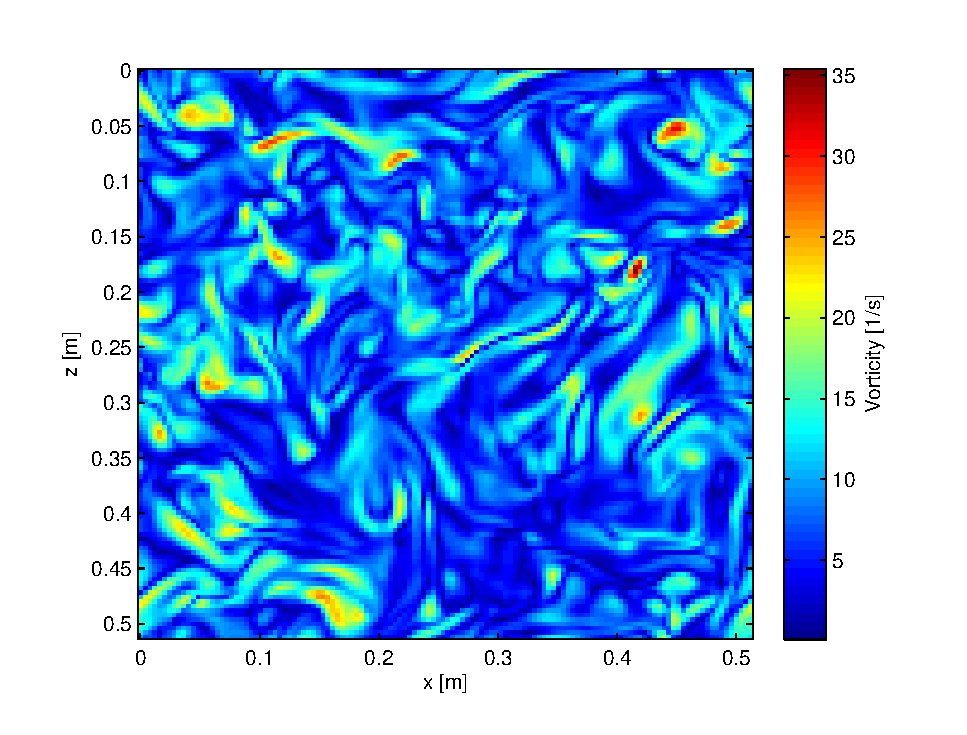
\includegraphics[width=0.48\textwidth]{Figures/vortex-1}

\caption{initial and final vorticity field ($1/s$) in x-z cross-sectional
plane for forced cases\label{fig:vort}}
\end{figure}